\section{Approach}
\label{sec:approach}

\begin{figure*}[t]
\centering
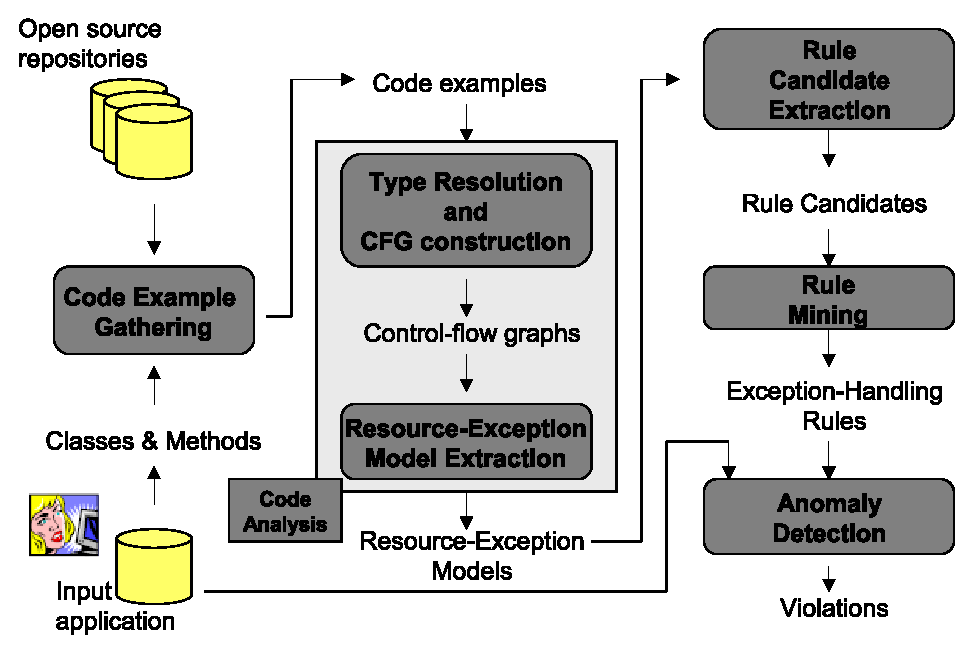
\includegraphics[scale=0.75,clip]{figs/architecture1.eps}\vspace*{-1ex}
\caption{Overview of our $\smoot$ approach.} \label{fig:architecture}
\vspace*{-3ex}
\end{figure*}

Figure~\ref{fig:architecture} shows a high-level overview of our $\smoot$ approach. $\smoot$ accepts an application under test and identifies classes and interfaces, declared or used by the application under test. These applications under test can also be frameworks or libraries. We refer to extracted classes for which sequences need to be collected as target classes, denoted by \{$TC_1$, $TC_2$, ..., $TC_m$\}. $\smoot$ also accepts a set of existing code bases, denoted by \{$CB_1$, $CB_2$, ..., $CB_n$\}, that already use these target classes. In our prototype implemented for the $\smoot$ approach, these code bases are in the form of .NET assemblies. Initially, $\smoot$ searches for relevant method bodies by using target classes as keywords. $\smoot$ constructs control-flow graphs for these method bodies and extracts sequences that produce objects of target classes. $\smoot$ extracts sequences by traversing these control-flow graphs. These extracted  sequences are used to assist random and DSE-based approaches. For DSE-based approaches, $\smoot$ converts extracted sequences into skeletons by replacing constant values for primitive types with symbolic values. We next explain each phase of MSeqGen in detail using the illustrative example shown in Figure~\ref{fig:mut}.

\begin{figure}[t]
\begin{CodeOut}
\begin{alltt}
00:public void Sort(VertexAndEdgeProvider vo) \{
01:\hspace*{0.1in}AdjacencyGraph g = new AdjacencyGraph(vo, true);
02:\hspace*{0.1in}Hashtable iv = new Hashtable();			
03:\hspace*{0.1in}int i = 0;  //adding vertices
04:\hspace*{0.1in}IVertex a = g.AddVertex();
05:\hspace*{0.1in}iv.Add(a);
06:\hspace*{0.1in}IVertex b = g.AddVertex();
07:\hspace*{0.1in}iv.Add(b);
08:\hspace*{0.1in}IVertex c = g.AddVertex();
09:\hspace*{0.1in}iv.Add(c);
10:\hspace*{0.1in}g.AddEdge(a,b);	//adding edges
11:\hspace*{0.1in}g.AddEdge(a,c);
12:\hspace*{0.1in}g.AddEdge(b,c);
13:\hspace*{0.1in}//TSAlgorithm: TopologicalSortAlgorithm
14:\hspace*{0.1in}TSAlgorithm topo = new TSAlgorithm(g);
15:\hspace*{0.1in}topo.Compute(); ... \}
\end{alltt}
\end{CodeOut}\vspace*{-3ex}
\Caption{\label{fig:adjacencyEx} A relevant method body for classes \CodeIn{AdjacencyGraph}, \CodeIn{VertexAndEdgeProvider}, \CodeIn{Hashtable}, and \CodeIn{TopologicalSortAlgorithm}.}\vspace*{-3ex}
\end{figure}

%-------------------------------------------------------------------------------
\subsection{Code Searching} 

We use code searching in our approach since code bases are often large and analyzing complete code bases can be prohibitively expensive. To avoid analyzing complete code bases, we use a keyword search to identify relevant method bodies including target classes. In particular, we use a text-based search, where the text is derived by decompiling .NET assemblies taken as inputs. We consider that a method body is relevant to a target class $TC_j$, if the method body includes the name of the $TC_j$ target class. For example, we use \CodeIn{AdjacencyGraph} as a keyword and search for method bodies including that keyword. Figure~\ref{fig:adjacencyEx} shows an example method body including the \CodeIn{AdjacencyGraph} keyword. As our code search is primarily a text-based search, code searching also returns irrelevant method bodies such as method bodies that include \CodeIn{AdjacencyGraph} as a variable name or a word in comments. We filter out such irrelevant method bodies in subsequent phases. 

We use intra-procedural analysis to analyze only such relevant method bodies. We use intra-procedural analysis since this analysis is more scalable than inter-procedural analysis. Although intra-procedural analysis is less precise than inter-procedural analysis, we address this precision issue by using an iterative strategy explained in subsequent sections. 

%TODO : Add more arguments of why we used intra-procedural analysis.

%-------------------------------------------------------------------------------
\subsection{Code Analysis} 

We next analyze each relevant method body statically and construct a control-flow graph (CFG). Our CFG includes four
types of statements: method calls, object creations, typecasts, and field accesses. The rationale behind choosing these statements is that these statements result in generating objects of target classes. While constructing a CFG, we identify the nodes (in the constructed CFG) that produce the target classes such as \CodeIn{AdjacencyGraph} and mark them as \emph{nodes of interest}. For example, the node corresponding to Statement 1 in Figure~\ref{fig:adjacencyEx} is marked as a node of interest for the target class \CodeIn{AdjacencyGraph}. We also filter out irrelevant method bodies identified during the code searching phase if their related CFGs do not contain any nodes of interest.

We next extract sequences from a CFG using nodes of interest. For each node of interest related to a target class $TC_j$, we gather a path from the node of interest to the end of the CFG. In the case of loops, we consider the nodes inside a loop as a group of nodes that is executed either once or not. Considering these nodes once can help identify the sequence inside the loop. We also annotate these nodes to store the additional information that these nodes (and their associated method calls) exist inside loops. This additional information is used in subsequent phases while generating code based on extracted sequences.

Often, an extracted sequence can include a few method calls that are unrelated to the target class $TC_j$. We use data-dependency analysis to filter out such unrelated method calls from the extracted sequence. We start with the method call (in short as \emph{base method call}) associated with a node of interest and filter out method calls that do not share the same receiver object as the base method call. Our data-dependency analysis results in a sequence that creates and mutates an object of a target class $TC_j$. For example, Figure~\ref{fig:agraphseq} shows a sequence gathered from the code example in Figure~\ref{fig:adjacencyEx}. $\smoot$ extracts several such  sequences for different classes from the same code example. For example, if the set of target classes also includes classes \CodeIn{Hashtable} and \CodeIn{TSAlgorithm}, $\smoot$ automatically extracts one  sequence for each of these classes as shown below from the code example. 

\begin{CodeOut}
\begin{alltt}
\emph{Sequence for Hashtable}:
\hspace*{0.3in}IVertex a,b,c; //requires as input
\hspace*{0.3in}Hashtable iv = new Hashtable();
\hspace*{0.3in}iv.Add(a);
\hspace*{0.3in}iv.Add(b);
\hspace*{0.3in}iv.Add(c);

\emph{Sequence for TSAlgorithm}:
\hspace*{0.3in}AdjacencyGraph g; //requires as input
\hspace*{0.3in}TSAlgorithm tsObj = new TSAlgorithm(g);
\hspace*{0.3in}tsObj.compute();
\end{alltt}
\end{CodeOut}

%\textbf{Handling new non-primitive types.} 
One issue with extracted sequences is that these sequences can include additional non-primitive types. For example, the  sequence for \CodeIn{AdjacencyGraph} (shown in Figure~\ref{fig:agraphseq}) requires non-primitive type \CodeIn{VertexAndEdgeProvider}. To achieve target states, we need new sequences for generating these additional non-primitive types. In principle, call sites in code bases including sequences for a $TC_j$ target class also include the sequences for generating related additional non-primitive types. However, in practice, often these call sites do not include sequences for these additional non-primitive types due to two factors. (1) A sequence for an additional non-primitive type is available in another method body and is not found by our approach as it uses intra-procedural analysis for extracting sequences.  (2) A sequence for an additional non-primitive type does not exist in the current code base $CB_i$ (such as a framework or a library) and expects a reusing application to provide a necessary sequence. 

We address this issue by extracting new sequences for additional non-primitive types by using an iterative strategy. More specifically, we first extract sequences for the initial set of target classes and collect all additional classes for which new sequences need to be extracted. We next extract sequences for these additional classes and collect more new additional classes. We repeat this process either till no new additional classes are collected or we reach a fixed number of iterations accepted as a configuration parameter, denoted by \emph{NUM\_ITERATIONS}. A high value for \emph{NUM\_ITERATIONS} can help collect more sequences; however, a high value can require more time for collecting those sequences. In our approach, we use five as the value of \emph{NUM\_ITERATIONS}, which is set based on our initial empirical experience.

%-----------------------------------------------------------------------
\subsection{Method-Call Sequence Generalization}

\begin{figure}[t]
\begin{CodeOut}
\begin{alltt}

\emph{A. Class Definition}:
00:class MyClass \{ 
01:\hspace*{0.1in}private int testMe;	
02:\hspace*{0.1in}private String ipAddr;	
03:\}

\emph{B. MUT}:
00:public void Mut1(MyClass mc, String IPAddress) \{
01:\hspace*{0.1in}if(mc.getTestMe() > 100) \{ 
02:\hspace*{0.2in}if(IsAValidIPAddress(IPAddress)) \{ ... \}
03:\hspace*{0.1in}\}
04:\}

\emph{C. Method-call sequence (MCS)}:
00:MyClass mcObj = new MyClass();
01:mcObj.SetTestMe(10);
02:mcObj.SetIpAddr("127.0.0.1");

\emph{D. Skeleton}:
00:int symvar = *, string ipaddr = *; 
01:MyClass mcObj = new MyClass();
02:mcObj.SetTestMe(symvar);
03:mcObj.SetIpAddr(ipaddr);

\end{alltt}
\end{CodeOut}\vspace*{-5ex}
\Caption{\label{fig:seqgeneralization} An illustrative example for method-call sequence generalization.}\vspace*{-3ex}
\end{figure}

%\emph{E. Skeleton with a boolean switch}:
%00:int symvar = *, string ipaddr = *; boolean bSymSwitch = *;
%01:if(bSymSwitch) \{
%02:\hspace*{0.1in}MyClass mcObj = new MyClass();
%03:\hspace*{0.1in}mcObj.SetTestMe(symvar);
%04:\hspace*{0.1in}mcObj.SetIpAddr(ipaddr);
%05:\} else \{
%06:\hspace*{0.1in}MyClass mcObj = new MyClass();
%07:\hspace*{0.1in}mcObj.SetTestMe(10);
%08:\hspace*{0.1in}mcObj.SetIpAddr("127.0.0.1");
%09:\}

We generalize sequences to address an issue that constant values in extracted sequences can be different from values required to achieve target states. We refer to the process of converting sequences into skeletons (which are sequences with symbolic values instead of concrete values for primitive types) as \emph{sequence generalization}. For example, consider a simple MUT and an example sequence (denoted as MCS) shown in Figures~\ref{fig:seqgeneralization}a to \ref{fig:seqgeneralization}c, respectively. The sequence cannot directly achieve the \CodeIn{true} branch of the MUT since the value of \CodeIn{testMe} is set to 10. To address this issue, we generalize extracted sequences. More specifically, we replace constant values of primitive types in extracted sequences with symbolic values. Figure~\ref{fig:seqgeneralization}d also shows the skeleton, where a symbolic variable \CodeIn{symvar} of type \CodeIn{int} is taken as input for the sequence. This \CodeIn{symvar} variable replaces the constant value 10 in the MCS. When this skeleton is used along with a DSE-based approach, the DSE-based approach initially generates a concrete random value for the \CodeIn{symvar} symbolic variable and gathers the constraint ($>$ $100$) in the MUT through dynamic execution. The DSE-based approach next solves the constraint to generate another concrete value for \CodeIn{symvar} such as $200$ that satisfies the gathered constraint. 

Although DSE-based approaches are effective in practice, it is challenging for these approaches to generate concrete values for variables that require complex values such as doubles, IP addresses, or URLs. In such cases, constant values in extracted sequences are useful in quickly covering those related branches such as the \CodeIn{true} branch in Statement 2 (Figure~\ref{fig:seqgeneralization}b) of the MUT. To address this issue, we preserve constant values in sequences along with the newly introduced symbolic values by using a symbolic \CodeIn{boolean} value as a switch between symbolic and constant values.
%TODO: Put a component called CodeGenerator. Show how we generate code automatically for Randoop and Pex. Also show how we handle loops.
%-----------------------------------------------------------------------
\subsection{Generation of New Sequences}

$\smoot$ extracts sequences from code bases and uses these sequences to assist random and DSE-based approaches. However, in some cases, these extracted sequences individually are not sufficient to achieve target states. $\smoot$ tries to address this issue by generating new sequences from extracted sequences by combining extracted sequences randomly. For example, consider two target classes $T_i$ and $T_j$, where $T_j$ requires an object of $T_i$ and a MUT requires an object of $T_j$. Consider that $\smoot$ identified two method bodies, denoted by $MD_1$ and $MD_2$, in code bases relevant to both $T_i$ and $T_j$. Consider that $\smoot$ extracted sequences $S_i^1$ and $S_j^1$ for target classes $T_i$ and $T_j$ from $MD_1$, respectively. Similarly, $\smoot$ extracted sequences $S_i^2$ and $S_j^2$ for target classes $T_i$ and $T_j$ from $MD_2$, respectively. The target class $T_i$ has sequences $S_i^1$ and $S_i^2$, and the target class $T_j$ has sequences $S_j^1$ and $S_j^2$. Given these sequences, $\smoot$ can generate some or all of four different combinations of these sequences for generating objects of $T_j$. These new sequences may further help achieve target states in the MUT.

\Comment{
For example, consider the following code example that includes two method bodies relevant to target classes \CodeIn{A} and \CodeIn{B}.

\begin{CodeOut}
\begin{alltt}
public void t1() \{
\hspace*{0.3in}A aobj = new A();
\hspace*{0.3in}aobj.ma1();
\hspace*{0.3in}B bobj = new B(aobj);
\hspace*{0.3in}bobj.mb1();
\}

public void t2() \{
\hspace*{0.3in}A aobj = new A();
\hspace*{0.3in}aobj.ma2();
\hspace*{0.3in}B bobj = new B(aobj);
\hspace*{0.3in}bobj.mb2();
\}
\end{alltt}
\end{CodeOut}

$\smoot$ extracts two  sequences each for classes \CodeIn{A} and \CodeIn{B} from the preceding code example. Extracting such individual  sequences can help generate new sequences such as a sequence including method calls \CodeIn{A.ma1} and \CodeIn{B.mb2}. These new sequences cannot be computed when long sequences with multiple classes are extracted. Our approach computes these combinations randomly.}
